\documentclass{beamer}
\usepackage{graphicx}
\usepackage[utf8]{inputenc}
\usepackage{biblatex}
\usepackage{marvosym}
\usepackage{booktabs}
\usepackage{multicol}
\usepackage{tabularx}
\setbeamercovered{transparent=15}
\addbibresource{../bibliography.bib}

\setbeamerfont{institute}{size=\large}
\setbeamerfont{date}{size=\small}

\newcommand\red[1]{\textcolor{red}{#1}}

\usetheme{Madrid}
\usecolortheme{orchid}

%\AtBeginSection[]{
%  \begin{frame}
%  \vfill
%  \centering
%  \begin{beamercolorbox}[sep=8pt,center,shadow=true,rounded=true]{title}
%    \usebeamerfont{title}\insertsectionhead\par%
%  \end{beamercolorbox}
%  \vfill
%  \end{frame}
%}
\AtBeginSubsection[]{
  \begin{frame}[allowframebreaks,noframenumbering]
    \frametitle{\contentsname}
    \begin{multicols}{2}
        \tableofcontents[currentsection,currentsubsection]
    \end{multicols}
  \end{frame}
}


\title{Blockchain and Bitcoin}
\subtitle[]{Overview of Blockchain technology and cryptocurrencies, focusing on
the Bitcoin protocol and its scalability and privacy aspects}
\institute[]{Università degli studi di Brescia}
\author{Michele Zanotti}
\date{18 Febbraio 2019}

\begin{document}
  \begin{frame}
    \titlepage
  \end{frame}
  \begin{frame}{Summary}
    \frametitle{\contentsname}
    \begin{multicols}{2}
        \tableofcontents
    \end{multicols}
  \end{frame}





  %%%%%%%%%%%%%%%%%%%%%
  %%% SECOND SECTION %%%
  %%%%%%%%%%%%%%%%%%%%%
  \section{Introduzione alle Blockchain}
  \subsection{Concetti preliminari}
 % \begin{frame}{Introduzione}
 %   \framesubtitle{Distributed systems}
 %   \begin{columns}[onlytextwidth]
 %     \column{.5\textwidth} \begin{block}{Distributed system}
 %       A \textcolor{red}{distributed system} is a network that %consists of autonomous nodes,
 %       connected using a distribution middleware, which acts in %a coordinated way
 %       (passing messages to each other) in order to achieve a %common outcome and
 %       that can be seen by the user as a single logical %platform.
 %     \end{block}

  %    \column{.5\textwidth}
  %    \begin{figure}[!htb]
  %      \centering
  %      \includegraphics[width=0.7\linewidth]{../img/distributed-%system.png}
  %    \end{figure}
  %  \end{columns}
  %\end{frame}




%  \begin{frame}{Introduzione}
%    \framesubtitle{Distributed systems}
%      The desired properties of a distributed system are the %following:\vspace{10pt}
%      \begin{itemize}
%        \item \textbf{Consistency}: all the nodes have the same %lates available copy of the data.
%        \item \textbf{Availability}: the system is always working %and responding to the
%        input requests without any failures.
%        \item \textbf{Partition tolerance}: if a group of nodes %fails the distributed system
%        still continues to operate correctly
%      \end{itemize}
%  \end{frame}


\begin{frame}{Introduzione}
    \begin{block}{Sistema distribuito}
    Un \textcolor{red}{sistema distribuito} è una rete composta da nodi autonomi, connessi attraverso un middleware, che operano in modo coordinato (scambiandosi messaggi) al fine di raggiungere un obiettivo comune e che possono essere visti dall'utente come singola piattaforma logica.  
    \end{block}
\end{frame}


  \begin{frame}{Introduzione}
    Anche se alcuni nodi/collegamenti si guastano, un sistema distribuito deve continuare a funzionare correttamente. Due tipi di guasto: 
    \begin{itemize}
      \item Semplice arresto del nodo
      \item Esibizione di comportamento maligno/inconsistente in modo arbitrario: \red{Byzantine fault}
    \end{itemize}

    \pause 
    \begin{block}{Byzantine nodes}
      Un \textcolor{red}{Byzantine node} è un nodo che manifesta un comportamento arbitrario, che può anche essere maligno. 
    \end{block}
  \end{frame}
  
  
  
  
  \begin{frame}{Introduzione}
        \begin{block}{Il problema dei generali Bizantini}
          \begin{itemize}
            \item Problema formulato da Leslie Lamport \cite{lamport1982byzantine}
            \item Un gruppo di generali sta circondando una città e deve concordare una decisione comune: attaccare o ritirarsi
            \item Il loro unico mezzo di comunicazione sono i messaggeri 
            \item Alcuni dei generali possono essere \emph{traditori}: possono comunicare messaggi fuorvianti al fine di impedire ai generali ``onesti'' di raggiungere un accordo comune
            \item Requisito: algoritmo che permetta ai generali onesti di concordare un piano comune, indipendentemente da quello che fanno i generali traditori
          \end{itemize}
        \end{block}
    \end{frame}

    \begin{frame}{Introduzione}
        \begin{figure}[!htb]
                \centering
                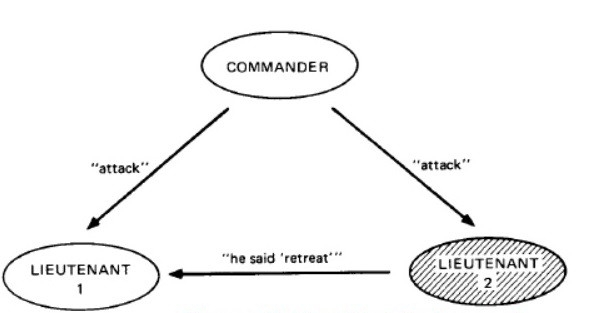
\includegraphics[width=0.5\linewidth]{../img/byzantine.jpg}
        \end{figure}
        \begin{figure}
            \centering
            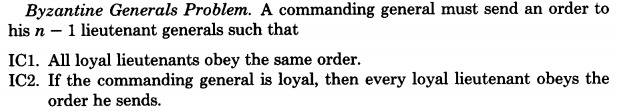
\includegraphics[width=0.7\linewidth]{../img/byzantine-generals-problem.png}
        \end{figure}
    \end{frame}




  \begin{frame}{Introduzione}
    \begin{block}{Consenso}
      \red{Consenso}: processo di accordo sul valore di un certo dato da parte di nodi che non si fidano tra di loro
    \end{block}

    \pause
    Requisiti per un algoritmo di Consenso:
    \begin{itemize}
      \item \textbf{Agreement}: i nodi non-Bizantini devono essere d'accordo sullo stesso valore
      \item \textbf{Termination}: l'algoritmo deve terminare (i nodi devono prendere una decisione)
      \item \textbf{Validity}: il valore concordato deve essere stato proposto da almeno un nodo \emph{onesto}
      \item \textbf{Fault tolerance}: l'algoritmo deve funzionare anche in presenza di nodi Bizantini 
    \end{itemize}
  \end{frame}

  
  
  
  \subsection{Definizione di Blockchain}
  \begin{frame}{Cosa è una Blockchain}
    \begin{block}{Business definition}
      Una Blockchain è una piattaforma dove è possibile scambiarsi valori (tra peers) senza il bisogno di una autorità centrale fidata, usando transazioni che vengono salvate all'interno della piattaforma stessa in modo verificabile e permanente. 
    \end{block}
    
    \pause
    \begin{block}{Definizione tecnica}
      Una Blockchain è un ``libro mastro'' distribuito (distributed ledger) che è:
      \begin{itemize}
        \item crittograficamente sicuro 
        \item append-only
        \item immutabile (estremamente difficile da modificare)
        \item aggiornabile solo attraverso consenso tra i nodi partecipanti
      \end{itemize}
    \end{block}
  \end{frame}



  \subsection{Caratteristiche}
  \begin{frame}{Caratteristiche di una Blockchain}
    \begin{itemize}
      \item \textbf{Decentralization}: non vi è il bisogno di una autorità centrale fidata che memorizzi e dati e validi le transazioni \pause
      \item \textbf{Distributed Consensus}: elevata tolleranza a Byzantine Faults, per ciascun dato vi è un'unica singola versione concordata da tutti i partecipanti attraverso un algoritmo di Consenso \pause
      \item \textbf{High availability}: Blockchain è basata su una rete peer-to-peer e i dati sono replicati su ciascun nodo: se anche un nodo si guasta, il sistema può continuare a funzionare correttamente
    \end{itemize}
  \end{frame}

  \begin{frame}{Caratteristiche di una Blockchain (Cont.)}
    \begin{itemize}
      \item \textbf{Immutability}: una volta che un blocco viene aggiunto alla Blockchain, modificarlo è computazionalmente impossibile \pause
      \item \textbf{Transparency}: ciascun nodo può vedere il contenuto della Blockchain \pause
      \item \textbf{Security}: integrità dei dati, autenticazione e non-ripudio sono garantiti. La privacy non è invece fornita. La sicurezza di una Blockchain è diretta conseguenza della sua natura distribuita
    \end{itemize}
  \end{frame}



  \subsection{Struttura}
  \begin{frame}{Struttura di una Blockchain}
    \begin{itemize}
      \item Lista ordinata di \red{blocchi} ordinati di dimensione prestabilita 
      \item Ciascun blocco contiene una lista di \red{transazioni}
    \end{itemize}

    \begin{figure}[!htb]
      \centering
      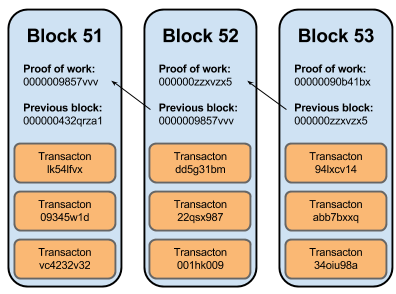
\includegraphics[width=0.45\linewidth]{../img/blockchain-basic-schema.png}
    \end{figure}
  \end{frame}




  \begin{frame}{Struttura di una Blockchain}
    \framesubtitle{Struttura di un blocco}
        \begin{figure}[!htb]
          \centering
          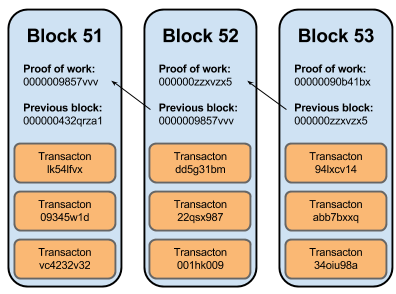
\includegraphics[width=0.3\linewidth]{../img/blockchain-basic-schema.png}
        \end{figure}
      \begin{itemize}
        \item  Un blocco è un insieme di transazioni. Generalmente, composto da:
        \begin{itemize}
          \item[-] un insieme di transazioni
          \item[-] una hash che identifica il blocco
          \item[-] un riferimento alla hash del blocco precedente
          \item[-] un nonce (numero casuale usato una sola volta)
          \item[-] un timestamp
        \end{itemize}
        \item Il primo blocco di una Blockchain viene chiamato \red{genesis block}.
      \end{itemize}
  \end{frame}




  \begin{frame}{Struttura di una Blockchain}
    \framesubtitle{Elementi caratteristici: nodi, indirizzi e transazioni}
    \begin{itemize}
      \item \textbf{Nodi} entità attive che mantengono una copia della Blockchain e che possono effettuare e/o validare transazioni \pause
      \item \textbf{Indirizzi} identificatori univoci che identificano le parti coinvolte in una transazione. Generalmente sono chiavi pubbliche (o sono derivati da chiavi pubbliche) \pause
      \item \textbf{Transazioni} trasferimenti di valore da un indirizzo all'altro \pause
      %\item \textbf{Transaction scripts} set di comandi predefiniti utilizzati dai nodi per trasferire valori da un nodo all'altro (es. possono definire le condizioni sotto cui un valore trasferito può essere utilizzato dal destinatario)
    \end{itemize}
  \end{frame}



  \subsection{Consenso}
  \begin{frame}{Consenso all'interno di Blockchain}
      \begin{itemize}
        \item Necessario per stabilire se i nuovi blocchi (o il libro mastro stesso) sono validi o no
        \item Analogia con il problema dei generali Bizantini:
        \begin{itemize}
            \item[-]i ``generali'' sono i nodi della Blockchain
            \item[-]i ``messengers'' sono i collegamenti tra i nodi della rete
            \item[-]i ``traditori'' sono i nodi maligni che cercano di manomettere i dati memorizzati nella blockchain
        \end{itemize} 
      \end{itemize}
  \end{frame}
  
  
  
  \begin{frame}{Consenso in Blockchain}
      Meccanismi di consenso comunemente usati in Blockchain: 
      \begin{enumerate}
        \item Practical Byzantine Fault Tolerance (\textbf{PBFT})
        \item Proof of Work (\textbf{PoW})
        \item Proof of Stake (\textbf{PoS})
        \item Delegated Proof of Stake (\textbf{DPoS})
      \end{enumerate}
  \end{frame}




  \begin{frame}{Consenso in Blockchain}
    \framesubtitle{Meccanismi di consenso comuni}
    \begin{block}{1) Practical Byzantine Fault Tolerance}
      \begin{itemize}
        \item Algoritmo proposto da M. Castro e B. Liskov. Versione ottimizzata della soluzione al problema dei generali Bizantini proposta da Lamport \cite{castro1999practical} 
        \item Ciascun ``generale'' mantiene uno stato interno. Quando riceve un messaggio, utilizza lo stato per eseguire una computazione che indica cosa pensare del messaggio in questione 
        \item Dopo aver raggiunto la sua conclusione individuale riguardo al messaggio ricevuto, il generale condivide tale conclusione con gli altri generali del sistema
        \item Decisione finale determinata in base alle decisioni presentate dai singoli generali \pause
        \item \textcolor{green}{Pro}: molto efficiente \pause
        \item \red{Cons}: preclude l'anonimità degli utenti \pause
        \item Meccanismo adottato da Hyperledger e Ripple
      \end{itemize}
    \end{block}
  \end{frame}




  \begin{frame}{Consenso in Blockchain}
    \framesubtitle{Meccanismi di consenso comuni}
    \begin{block}{2) Proof of Work}
      \begin{itemize}
        \item Contrariamente a PBFT, non richiede che tutti i nodi presentino le loro conclusioni individuali 
        \item È basato su una ``prova'' che assicura che sufficienti risorse computazionali siano state spese da parte del nodo prima di proporre un nuovo blocco alla rete (il quale gli altri nodi decideranno se accettare come valido)
        \item Solamente un singolo nodo annuncia il blocco (il primo che risolve la PoW) 
        \item Il blocco annunciato può essere indipendentemente verificato da tutti gli altri nodi \pause
        \item Meccanismo utilizzato da Bitcoin
      \end{itemize}
    \end{block}
  \end{frame}





  \begin{frame}{Consenso in Blockchain}
    \framesubtitle{Meccanismi di consenso comuni}
    \begin{block}{3) Proof of Stake}
      \begin{itemize}
        \item Per proporre un nuovo blocco non è necessario portare a termine una prova che richieda calcolo intensivo
        \item Per decidere chi annuncierà il prossimo blocco, la rete esegue una ``lotteria'' basata sull'interesse (stake) dei singoli nodi
        \begin{itemize}
            \item[\MVRightarrow] e.g. stake = quantità di denaro depositata dal nodo
            \item[\MVRightarrow] se un nodo approva transazioni non valide perde il suo stake
        \end{itemize}
        \item Maggiore stake un nodo ha, maggiori sono le probabilità che esso verrà scelto 
        \item \textcolor{green}{Idea principale}: validatori hanno elevato stake \MVRightarrow azione maligne non garantisce abbastanza benefici \pause
        \item \red{Problema principale}: maggiori ricompense a coloro che hanno maggiore stake \MVRightarrow\ il sistema tende a divenire sempre più centralizzato
      \end{itemize}
    \end{block}
  \end{frame}





  \begin{frame}{Consenso in Blockchain}
    \framesubtitle{Meccanismi di consenso comuni}
    \begin{block}{4) Delegated Proof of Stake}
      \begin{itemize}
        \item Evoluzione di PoS
        \item Utilizza un sistema di votazione per eleggere delegati che valideranno i nuovi blocchi 
        \item Maggiore stake uno nodo ha, maggiore è il valore del suo voto 
        \item Il processo di votazione è eseguito periodicamente: se i delegati non si comportano correttamente, gli altri nodi non li voteranno più
        \item Ciascun nodo può delegare il proprio stake ad un altro stakeholder (che voterà a suo nome) 
        \end{itemize}
    \end{block}
  \end{frame}



  \subsection{Tipi di Blockchain}
  \begin{frame}{Tipi di Blockchain}
    \begin{block}{1) Public Blockchain}
      \begin{itemize}
        \item Blockchain publiche, chiunque può unirsi alla rete, mantenere una copia del libro mastro e partecipare al processo di Consenso 
        \item Il libro mastro non è posseduto da alcuna entità, chiunque può leggerlo
        \item Solitamente vi sono incentivi per incoraggiare nuovi partecipanti ad unirsi alla rete \pause
        \item \red{Principale problema}: mancanza di privacy (chiunque può vedere tutte le transazioni) \pause
        \item Bitcoin si basa su una Blockchain pubblica
      \end{itemize}
    \end{block}
  \end{frame}




  \begin{frame}{Tipi di Blockchain (Cont. 1)}
    \begin{block}{2) Private Blockchain}
      \begin{itemize}
        \item Aperte solo a una determinata organizzazione o a un certo gruppo di individui
        \item Per partecipare alla rete e mantenere una copia del libro mastro, i partecipanti devono ricevere un invito/permesso
        \begin{itemize}
            \item[\MVRightarrow] autorità centrale
        \end{itemize}
        \item Solitamente la rete è permissionata: restrizioni su chi può partecipare e su cosa può fare
        \item Esempio di private Blockchain: Hyperledger Fabric \cite{hyperledger-fabric}
      \end{itemize}
    \end{block}
  \end{frame}




  \begin{frame}{Tipi di Blockchain (Cont. 2)}
    \begin{block}{3) Consortium Blockchain}
      \begin{itemize}
        \item Il processo di Consenso è controllato da un gruppo di nodi preselezionati (e.g. un consorzio di organizzazioni, ciascuna delle quali controlla un nodo) 
        \item Il permesso di lettura del libro mastro può essere ristretto o libero 
        \item Esempio di consortium Blockchain: R3 \cite{R3}
      \end{itemize}
    \end{block}
  \end{frame}










  %%%%%%%%%%%%%%%%%%%%%
  %%% THIRD SECTION %%%
  %%%%%%%%%%%%%%%%%%%%%
  \section{Bitcoin}
  \subsection{Cosa è Bitcoin}
  \begin{frame}{Cosa è Bitcoin}
    \begin{itemize}
      \item Prima crittovaluta completamente decentralizzata
      \item Inventato da Satoshi Nakamoto nel 2008: prima vera implementazione di una Blockchain
      \item Bitcoin può essere definito sia come protocollo, valuta digitale e piattaforma
    \end{itemize}

   % \begin{block}{L'implementazione di riferimento}
%      \begin{itemize}
%        \item Bitcoin è un progetto Open Source ed è %sviluppato da una comunità di volontari
%        \item L'implementazione di riferimento (nonchè la %più usata) \textbf{Bitcoin Core}
%        \item È considerata l'implementazione %``autoritativa'' e specifica come ciascuna parte del %sistema debba essere implementata
%        \item Esistono diversi Bitcoin client alternativi %a Bitcoin Core
%        \begin{itemize}
%%            \item[\MVRightarrow] implementazioni non a%utoritative
 %       \end{itemize}
 %     \end{itemize}
 %   \end{block}
  \end{frame}




  \begin{frame}{Cosa è Bitcoin (Cont. 1)}
    Bitcoin può essere visto come una combinazione di: 
    \begin{itemize}
      \item rete peer-to-peer decentralizzata (il protocollo Bitcoin)
      \item un libro mastro pubblico e aperto a tutti (la Blockchain) 
      \item un insieme di regole per validare le transazioni  
      \item un meccanismo di Consenso (un algoritmo distribuito di Consenso) 
    \end{itemize}
  \end{frame}





  \begin{frame}{Cosa è Bitcoin (Cont. 2)}
    I bitcoins sono interamente ``virtuali'': 
    \begin{itemize}
      \item non vi è alcuna moneta fisica o digitale
      \item i coins sono impliciti nelle transazioni 
    \end{itemize}
  \end{frame}





  \subsection{Scripts}
  \begin{frame}{Bitcoin scripts}
    \begin{itemize}
      \item Script = lista di istruzioni registrate con ciascuna transazione che specificano come il prossimo utente che vuole spendere i bitcoin trasferiti può accedervi (e spenderli) \pause 
      \item Linguaggio di programmazione utilizzato: ``\red{Script}'' \cite{script-bitcoin-wiki} 
      \begin{itemize}
        \item linguaggio molto semplice 
        \item non Turing-complete {\tiny(no loops and no complex control flow instructions)} 
        \item deliberatamente progettato per evitare abusi degli script volti a condurre attacchi Denial of Service {\tiny(ciascuno script deve essere eseguito ciascun nodo della rete)}
      \end{itemize}
    \end{itemize}
  \end{frame}




  \subsection{Chiavi e Indirizzi}
  \begin{frame}{Chiavi e Indirizzi}
    \begin{itemize}
      \item Il possesso di bitcoin è stabilito tramite:
      \begin{itemize}
          \item chiavi crittografiche 
          \item indirizzi Bitcoin 
          \item firme digitali
      \end{itemize} 
      \item Per essere inclusa nella Blockchain, una transazione richiede una firma valida, la quale può essere generata solo attraverso una chiave privata (segreta)  
      \begin{itemize}
          \item prova il possesso dei bitcoin
%          \item non ripudio
      \end{itemize}
    \pause
    \end{itemize}
    \begin{block}{Analogia con le banche tradizionali}
      \begin{itemize}
        \item chiave pubblica \MVRightarrow\, numero del conto bancario
        \item chiave privata \MVRightarrow\, PIN segreto (o firma su un assegno) che permette di ``sbloccare'' il valore e trasferirlo ad altre persone 
      \end{itemize}
    \end{block}
  \end{frame}





  \begin{frame}{Chiavi e Indirizzi (Cont. 1)}
    \begin{block}{Indirizzi}
      \begin{itemize}
        \item indirizzo = stringa univoca di lettere e cifre che identifica il mittente o il destinatario di una transazione  \pause
        \item derivate dalle chiavi pubbliche attraverso hashing one-way:
        \begin{enumerate}
          \item Double hashing: SHA-256 + RIPEMD160
          \item hash di 160-bit come risultato
          \item Base58Check encoding of the 160-bit hash
          \item Risultato: stringa di 26-35 charatteri che inizia con ``1'' (\red{public key address}) o con ``3'' (\red{pay-to-script-hash address})
        \end{enumerate}
      \end{itemize}
    \end{block}
  \end{frame}





  \begin{frame}{Chiavi e Indirizzi (Cont. 2)}
    \begin{block}{Chiavi}
      \begin{itemize}
        \item \textbf{Chiavi private}: numeri casuali di 256 bit \pause
        \item \textbf{Chiavi pubbliche}: generate partendo dalle chiavi private usando la moltiplicazione su curve ellittiche: \pause
        \begin{itemize}
          \item Funzione ``a botola'' 
          \item Curva ellittica specificata dallo standard secp256k1, definito dal NIST:
          \[ y^2 \bmod p = (x^3 + 7) \bmod p \]
          dove $p = 2^{256} – 2^{32} – 2^9 – 2^8 – 2^7 – 2^6 – 2^4 – 1$ è un numero primo molto grande 
          \item Chiave pubblica $K=k*G$, dove $k$ è la chiave privata e $G$ è un punto sulla curva definita dallo standard 
          \item Il punto generatore $G$ è sempre lo stesso per tutti gli utenti di Bitcoin
        \end{itemize}
      \end{itemize}
    \end{block}
  \end{frame}





  \begin{frame}{Chiavi e Indirizzi (Cont. 3)}
    \begin{block}{Formati delle chiavi pubbliche}
      \begin{itemize}
        \item \textbf{Formato non compresso}: la chiave corrisponde alle coordinate $(x,y)$ di un punto sulla curva \MVRightarrow\, prefisso $04$ seguito da due numeri da 256 bit (65 byte) \pause
        \item \textbf{Formato compresso}: prefisso $03$ (se la coordinata y è un numero dispari) o $02$ (se la coordinata y è un numero pari) seguito dalla coordinata x \MVRightarrow\, 33 Bytes
        \begin{itemize}
          \item la coordinata y può essere derivata da quella x \pause
        \end{itemize}
        \item indirizzo derivato da chiave compressa $\neq$ indirizzo derivato dalla versione non compressa \pause
        \begin{itemize}
          \item soluzione: \textbf{chiavi private compresse}
          \item chiavi private da cui solamente chiavi pubbliche in formato compresso possono essere derivate
        \end{itemize}
      \end{itemize}
    \end{block}
  \end{frame}




  \subsection{Transazioni}
  \begin{frame}{Transazioni}
    \begin{itemize}
      \item Strutture dati che contengono i valori trasferiti dai partecipanti all'interno del sistema Bitcoin
      \item Sono pubbliche e visibili a chiunque 
      \item Una transazione include almeno un input e almeno un output
    \end{itemize}
  \end{frame}





  \begin{frame}{Transazioni (Cont. 1)}
    \begin{block}{Outputs}
      \begin{itemize}
        \item L'output è composto da due parti:
        \begin{enumerate}
          \item una quantità di bitcoin (discreta e indivisibile, espressa in Satoshi) 
          \item un insieme di condizioni da soddisfare per poter spendere i bitcoin in output (\textbf{locking script})
        \end{enumerate}
        \pause
        \item Tutti gli output spendibili memorizzati all'interno della Blockchain vengono chiamati \textbf{UTXO} (Unspent Transaction Outputs)
        \item Saldo del Wallet = valore aggregato di tutti gli UTXOs che l'utente può spendere con le chiavi in suo possesso 
        \item Un UXTO può solo essere speso interamente
        \begin{itemize}
          \item[$\rightarrow$] normalmente le transizioni generano \emph{resto} in output
        \end{itemize}
      \end{itemize}
    \end{block}
  \end{frame}





  \begin{frame}{Transazioni (Cont. 2)}
    \begin{block}{Inputs}
      L'input di una transazione è composto da: 
      \begin{enumerate}
        \item uno o più UTXOs che verranno ``consumati''
        \item una prova che certifichi la proprietà degli UTXOs da consumare attraverso il locking script 
        \begin{itemize}
          \item[$\rightarrow$] normalmente si tratta di una firma digitale + relativa chiave pubblica 
        \end{itemize}
      \end{enumerate}
    \end{block}
  \end{frame}
  
  
  
  
  \begin{frame}{Transazioni (Cont. 3)}
    \begin{block}{Esempio di transazione}
        \textbf{Input}\\
        \begin{itemize}
            \item Previous tx: \begin{tiny}f5d8ee39a430901c91a5917b9f2dc19d6d1a0e9cea205b009ca73dd04470b9a6\end{tiny}
            \item Index: 0
            \item scriptSig: 
            \begin{enumerate}
                \item \begin{tiny}304502206e21798a42fae0e854281abd38bacd1aeed3ee3738d9e1446618c4571d10\end{tiny}
                \item \begin{tiny}90db022100e2ac980643b0b82c0e88ffdfec6b64e3e6ba35e7ba5fdd7d5d6cc8d25c6b241501\end{tiny}
            \end{enumerate}
        \end{itemize}

        \textbf{Output}\\
        \begin{itemize}
            \item Value: 5000000000
            \item scriptPubKey: OP\_DUP OP\_HASH160 \begin{tiny}i404371705fa9bd789a2fcd52d2c580b65d35549d\end{tiny}\\ OP\_EQUALVERIFY OP\_CHECKSIG
        \end{itemize}
    \end{block}
  \end{frame}
  
  
  
  
%  \begin{frame}{Transazioni (Cont. 4)}
%      \begin{figure}
%          \centering
%          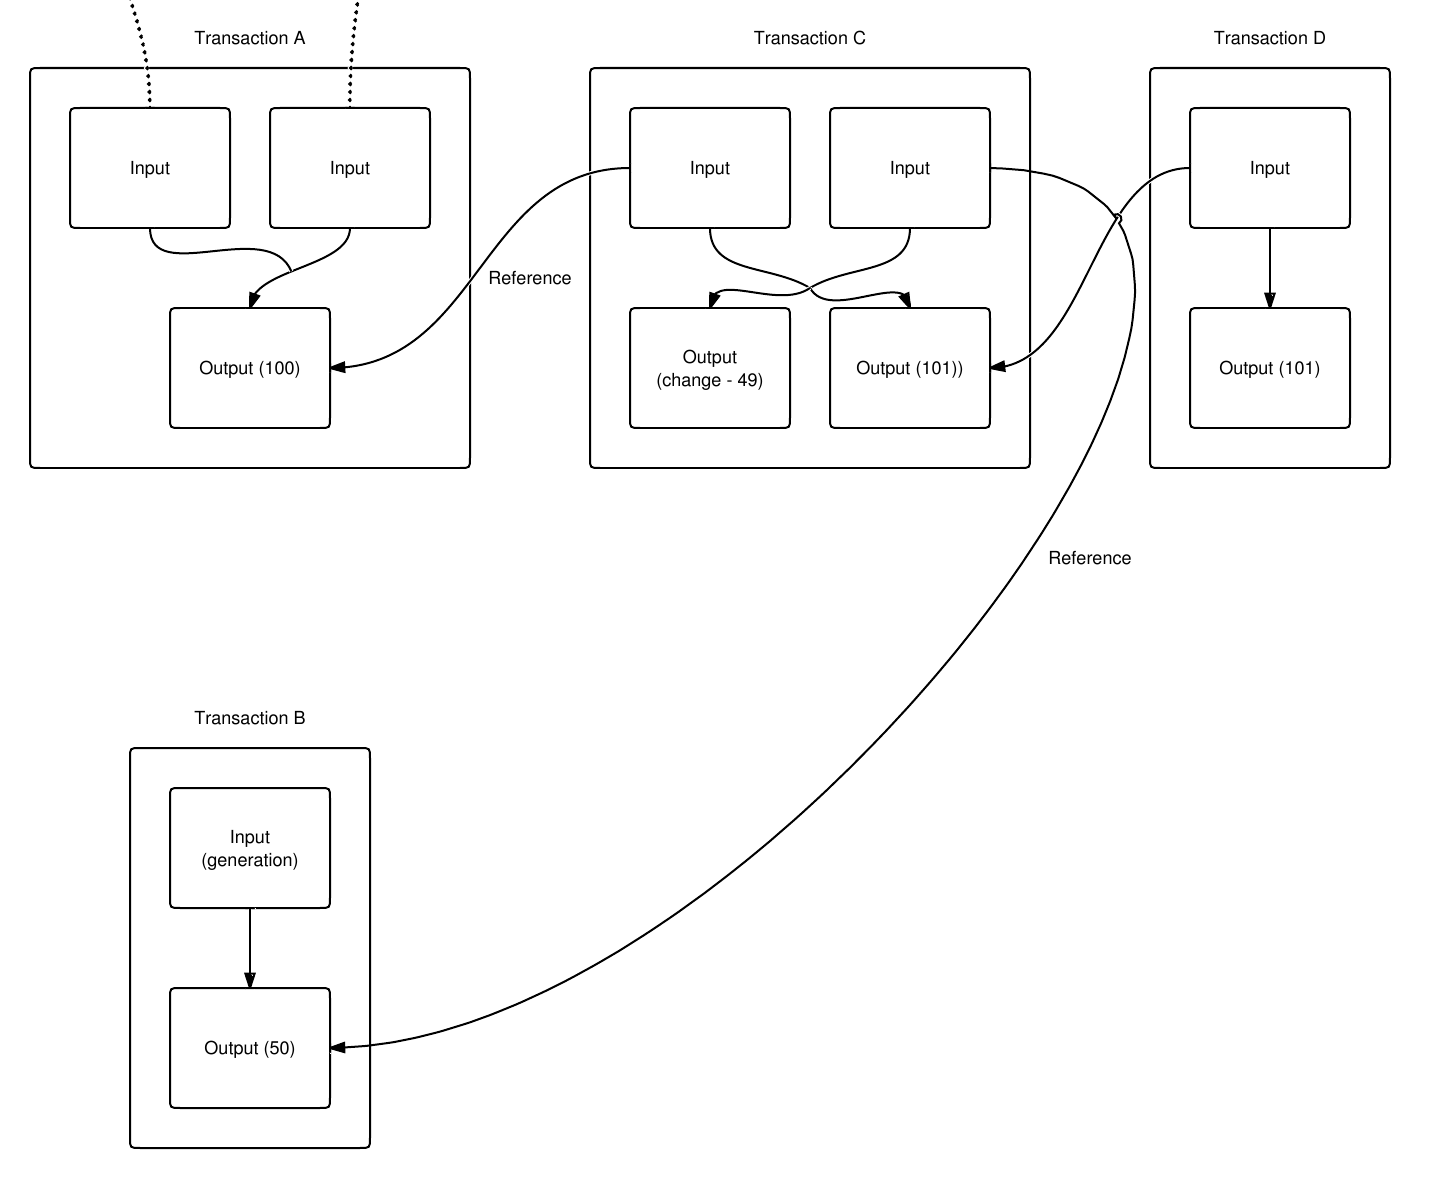
\includegraphics[width=0.8\linewidth]{../img/Transaction.png}
%      \end{figure}
%  \end{frame}





%  \begin{frame}{Transazioni (Cont. 3)}
%    \begin{block}{Transaction typical life cycle}
%      \begin{enumerate}
%        \item A sender sends a transaction (using a wallet application) 
%        \item The wallet signs the transaction using the sender’s private %key in order
%        to prove the ownership of the value being transferred 
%        \item The transaction is broadcasted to the Bitcoin network 
%        \item Mining nodes include this transaction in the next block to %be mined 
%        \item When a node solves the Proof of Work it broadcasts the
%        newly block to the network 
%        \item Confirmation process starts: each node verifies the new %block and propagate it further
%      \end{enumerate}
%    \end{block}
%  \end{frame}

  \begin{frame}{Transazioni (Cont. 4)}
    \begin{block}{Tasse sulle transazioni}
      \begin{itemize}
        \item Due scopi:
        \begin{enumerate}
          \item ricompensare i miner
          \item meccanismo di sicurezza: rendere economicamente impossibile per gli attaccanti inondare la rete di transazioni (DoS) 
        \end{enumerate}
        \item Il loro valore dipende dalla dimensione della transazione: 
        \[ Fees = Sum(Inputs)–Sum(Outputs) \] 
        \item Lo spender della transazioen è colui che decide il valore della tassa da pagare
        \begin{itemize}
            \item i miner scelgono da un pool le transazioni che includeranno nel prossimo blocco
            \item maggiori tasse = transazione confermata più velocemente (il blocco verrà minato prima) 
            \item tasse nulle = la transazione probabilmente non verrà mai confermata
        \end{itemize}
      \end{itemize}
    \end{block}
  \end{frame}





  \begin{frame}{Transazioni (Cont. 5)}
    \begin{block}{Transazione Coinbase}
      \begin{itemize}
        \item Prima transazione di ciascun blocco
        \item Creata dal primo nodo che risolve al Proof-Of-Work
        \item Genera nuovi bitcoin che il miner può spendere (ricompensa per aver minato il blocco)
        \item no UTXO in input: hanno un input speciale detto coinbase
      \end{itemize}
    \end{block}
  \end{frame}





  \subsection{Wallets}
  \begin{frame}{Wallets}
    \begin{itemize}
      \item Applicazioni che fungono da interfaccia utente e ne gestiscono il denaro 
      \item Def. tecnica: strutture dati che memorizzano in modo sicuro le chiavi private dell'utente richieste per spendere i bitcoin che gli possiede 
      \item Non memorizzano ``denaro'', ma solamente coppie di chiavi pubbliche/private
      \item Due tipi di wallet: \emph{deterministici} e \emph{non deterministici}
    \end{itemize}
  \end{frame}




%  \begin{frame}{Wallets (Cont. 1)}
%    \begin{block}{Wallet non deterministici}
%      \begin{itemize}
%        \item Ciascuna chiave è generata in modo indipendente a partire da un %numero casuale \MVRightarrow\, le chiavi memorizzate non sono connesse tra %loro in alcun modo
%        \item Principale svantaggio: ingombranti da gestire
%        \begin{itemize}
%          \item[-] richiesto backup frequente del wallet \MVRightarrow\, %backup di ciascuna chiave che contiene 
%          \item[-] utente evita di riutilizzare indirizzi \MVRightarrow\, %molti indirizzi \MVRightarrow\, molte chiavi di cui si deve fare il backup %frequentemente
%        \end{itemize}
%      \end{itemize}
%    \end{block}
%  \end{frame}




%  \begin{frame}{Wallets (Cont. 2)}
%    \begin{block}{Wallet deterministici}
%      \begin{itemize}
%        \item Tutte le chiavi vengono derivata da una singola chiave master %(detta \emph{seed}) 
%        \item Le chiavi memorizzate possono essere generate nuovamente se si %possiede il seed
%        \item Il backup riguarda solo il seed
%        \item Facili da gestire, anche quando si evita di riutilizzare gli %indirizzi
%        \item Le chiavi sono normalmente derivate in una struttura ad albero %(standard BIP-32) 
%        \begin{itemize}
%            \item elevata flessibilità
%        \end{itemize}
%        \item Seed normalmente creati come specificato dallo standard BIP-39 
%        \begin{itemize}
%          \item[-] sequenza di parole inglesi chiamate \emph{mnemonic} 
%          \item[-] facile da trascrivere, esportare e importare attraverso %diversi wallet
%        \end{itemize}
%      \end{itemize}
%    \end{block}
%  \end{frame}




  \subsection{Bitcoin Blockchain}
  \begin{frame}{Bitcoin Blockchain}
     \begin{itemize}
         \item Lista di blocchi di transazioni collegati tra loro
         \item Ciascun blocco identificato da una hash SHA-256
         \item Ciascun blocco include nell'header l'hash del blocco precedente
         \begin{itemize}
             \item modificare un blocco modifica anche la sua hash
             \item anche l'hash dei blocchi figli cambia (effetto cascata)
         \end{itemize}
     \end{itemize}
  \end{frame}
  
  
  
  \begin{frame}{Bitcoin Blockchain}
    \begin{figure}[!htb]
    \centering
    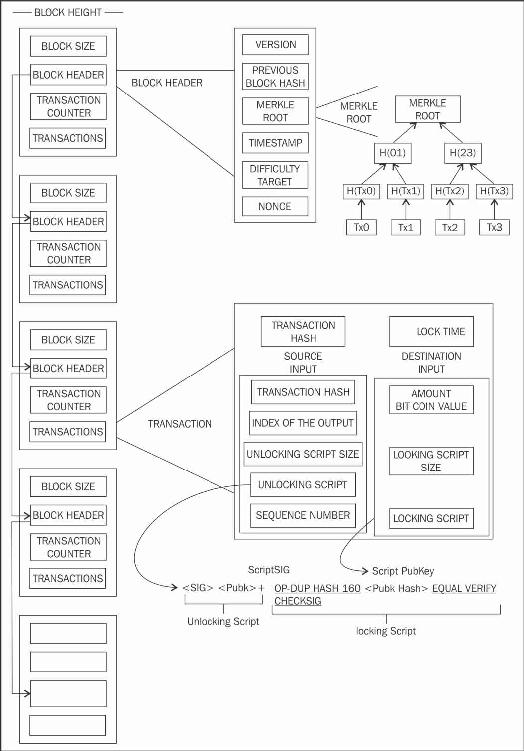
\includegraphics[width=0.45\linewidth]{../img/bitcoin-blockchain-scheme.png}
    \end{figure}
  \end{frame}
  
  
  
  \begin{frame}{Bitcoin Blockchain}
      \begin{block}{Alberi di Merkle}
          \begin{itemize}
              \item Strutture dati usate per riassumere e verificare l'integrità di grandi insiemi di dati in modo efficiente (alberi binari di hash)
              \item Utilizzati per verificare in modo efficiente se una certa transazione è inclusa in un certo blocco
              \item La radice dell'albero è memorizzata nell'header di ciascun blocco e riassume le transazioni incluse in esso
              \begin{itemize}
                  \item [\MVRightarrow] i nodi possono verificare le transazioni senza dover scaricare i blocchi interi (scaricano solo Merkle path + block header)
              \end{itemize} 
          \end{itemize}
      \end{block}
  \end{frame}
  
  
  
  \begin{frame}{Bitcoin Blockchain}
    \framesubtitle{Alberi di Merkle}
    \begin{figure}
      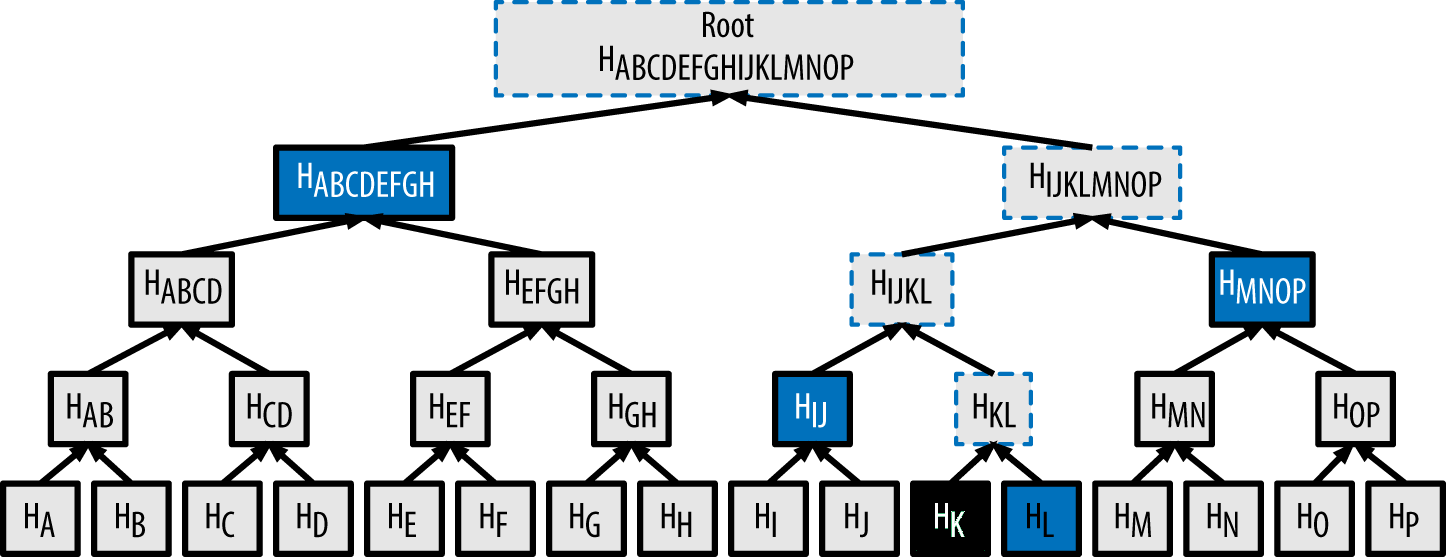
\includegraphics[width=0.6\linewidth]{../img/merkle-tree-path.png}
    \end{figure}
    \begin{itemize}
        \item Per verificare se una transazione è inclusa in un blocco, solo  $log_2(N)$ hash devono essere scaricate ($N$ numero di transazioni del blocco)
    \end{itemize}
  \end{frame}
  
  
  
  
  
  \begin{frame}{Bitcoin Blockchain}
  \framesubtitle{Alberi di Merkle}
      \footnotesize
       \begin{tabularx}{\textwidth}{l l l l}
         \toprule
         \textbf{Number of transactions}	& \textbf{Approx size of block} & \textbf{Path size} &	\textbf{Path size}   \\ \midrule
         16 transactions & 4 kilobytes & 4 hashes & 128 bytes \\
         \\
         512 transactions & 128 kilobytes & 9 hashes & 288 bytes \\
         \\
         2048 transactions & 512 kilobytes & 11 hashes & 352 bytes \\
         \\
         65535 transactions & 16 megabytes & 16 hashes & 512 bytes \\
         \bottomrule
     \end{tabularx}
  \end{frame}
  
  
  
  
  \subsection{Bitcoin Network}
  \begin{frame}{Bitcoin Network}
    Rete peer-to-peer:
    \begin{itemize}
        \item no nodi ``speciali'' (tutti i nodi utilizzano e forniscono servizi) 
        \item topologia ``flat''
        \item ciascun nodo connesso a pochi peers
        \begin{itemize}
            \item[\MVRightarrow] prevenzione di attacchi DoS  % otherwise a node could broadcast many bad-formed blocks/Transazioni
        \end{itemize}
    \end{itemize}
    
    Tre diversi tipi di nodi:
    \begin{enumerate}
        \item Full nodes
        \item Miners
        \item Lightweight clients
    \end{enumerate}
    
    %Despite the type, all the nodes validate and propagate blocks
  \end{frame}
  
  
  
  
  \begin{frame}{Bitcoin Network}
    \framesubtitle{Tipi di nodi}
    \begin{block}{1) Full nodes}
        \begin{itemize}
            \item Mantengono una copia dell'intera Blockchain
            \begin{itemize}
                \item[\MVRightarrow] possono autonomamente e autoritativamente verificare tutte le transazioni (possono ricostruire l'insieme degli UTXOs)
            \end{itemize}
            \item Validano e inoltrano transazioni/blocchi ai loro peer
            \item \textcolor{red}{Svantaggio}: la dimensione della Blockchain è attualmente di circa 178 GB \cite{statista}
            \item \textcolor{green}{Vantaggi}: 
            \begin{itemize}
                \item[-] contribuiscono alla sicurezza di Bitcoin
                \item[-] maggiore sicurezza (un full node può vedere tutte le transazioni), può verificare transazioni senza appoggiarsi a terze parti
            \end{itemize}
        \end{itemize}
    \end{block}
  \end{frame}
  
  
  
  
   \begin{frame}{Bitcoin Network}
    \framesubtitle{Tipi di Nodi}
    \begin{block}{2) Miners}
        \begin{itemize}
            \item Nodi che risolvono la proof-of-work e creano nuovi blocchi
            \item Competono tra di loro 
            \item Non devono necessariamente essere full-nodes
            \begin{itemize}
                \item[\MVRightarrow] partecipano a mining pool \footnote{Mining pool = gruppo di miners che cooperano tra loro e si spartiscono le ricompense in proporzione alla loro hash power messa a disposizione} in cui solo un server mantiene la copia completa della Blockchain
            \end{itemize}
        \end{itemize}
    \end{block}
  \end{frame}
  
  
  
  
  \begin{frame}{Bitcoin Network}
    \framesubtitle{Tipi di Nodi}
    \begin{block}{3) Lightweight clients}
        \begin{itemize}
            \item Clients progettati per essere eseguiti su device con risorse limitate (e.g. smartphones, tablets, etc.) 
            \item Memorizzano solo gli header dei blocchi 
            \item Validano le transazioni usando lo schema SPV (Simple Payment Verification) \footnote{e.g. verificano che nessuno degli input della transazione sia già stato precedentemente speso}
            \begin{itemize}
                \item[-] controllano che una transazione appartenga a un blocco richiedendo un Merkle Path ad un full node
                \item[-] verificano la proof-of-work del blocco
                \item[-] non ricostruiscono l'insieme degli UTXO: controllano quanto profondamente il blocco della transazione è ``sepolto'' \MVRightarrow\, molti blocchi sopra di esso = la transazione è valida (e.g. non è già stata spesa)
            \end{itemize}
        \end{itemize}
    \end{block}
  \end{frame}
  
  
  
  
  \begin{frame}{Bitcoin Network}
    \framesubtitle{Node types}
    \begin{block}{Svantaggi dei Lightweight Client}
        \begin{itemize}
            \item Devono fidarsi dei full nodes (assumono che i blocchi e le transazioni siano validati correttamente da quest'ultimi)
            \item Non possono verificare che una transazione \emph{non esiste} (possono solo verificare se \emph{esiste})
            \begin{itemize}
                \item[\MVRightarrow] possibilità di spendere una transazione due volte (spendere gli stessi UTXO due volte) nascondendo al nodo la prima transazione
                \pause
                \item[\MVRightarrow] \textcolor{green}{Soluzione}: i nodi SPV
                si connettono in modo casuale a diversi full node (maggiore possibilità di trovare almeno un nodo onesto) 
            \end{itemize}
        \end{itemize}
    \end{block}
  \end{frame}
  
  
  \subsection{Mining e Consenso}
  \begin{frame}{Mining e Proof of Work}
      \begin{itemize}
          \item Mining = processo attraverso il quale le transazioni sono validate e nuovi blocchi sono creati e aggiunti alla Blockchain
          \item Un nuovo blocco viene creato ogni circa 10 min 
          \item I miners sono ricompensati con basecoin + tasse
          \item Per creare un nuovo blocco, i miners devono risolvere la \textbf{Proof of Work}
      \end{itemize}
  \end{frame}
  
  
  
  \begin{frame}{Mining e Proof of Work}
      \begin{block}{Proof of Work}
      \begin{center}
          $H(N||Prev\_hash||Tx||Tx||....||Tx)<Target$
      \end{center}
        \begin{itemize}
            \item Problema difficile basato su un algoritmo crittografico di hash (SHA-256)
            \item Rappresenta la prova che il miner ha speso abbastanza abbastanza risorse computazionali
            \item Il target (la difficoltà) viene sempre aggiornata in modo che i blocchi vengano minati ogni circa 10 min
            \item L'hash $H$ è calcolata solo sull'header del blocco
            \item Dopo che un blocco è stato minato, il nodo lo trasmette a tutti i suoi peer
            \begin{itemize}
                \item[\MVRightarrow] i nodi lo validano e lo propagano a loro volta
            \end{itemize}
        \end{itemize}
      \end{block}
  \end{frame}
  
  
  
  \begin{frame}{Consenso}
    \begin{itemize}
        \item No autorità centrale
        \item \textbf{Consenso Emergente}: il consenso non viene raggiunto esplicitamente
        \item Il consenso emerge da:
        \begin{enumerate}
            \item verifica indipendente delle transazioni da parte dei nodi
            \item aggregazione delle transazioni in blocchi e risoluzione della PoW
            \item verifica indipendente dei nuovi blocchi minati 
        \end{enumerate}
        \item Un blocco ha più figli in cascata \MVRightarrow per modificarlo bisogna anche modificare tutti i blocchi successivi
         \begin{itemize}
             \item[\MVRightarrow] bisogna risolvere nuovamente la PoW 
             \item[\MVRightarrow] i blocchi sono praticamente immutabili
         \end{itemize}
        %\item A transaction is included in a block \MVRightarrow mined at a depth of 1 %\begin{itemize}
        %    \item subsequent block found \MVRightarrow the number of blocks deep is increased by 1
        %\end{itemize}
        \item Client Bitcoin classico:  ``unconfirmed'' fino a che la transazione è profonda 6 blocchi
    \end{itemize}
  \end{frame}
  
  
  
  
  \begin{frame}{Consenso}
      \begin{block}{Verifica delle transazioni}
      Il nodo controlla: 
        \begin{itemize}
            \item sintassi della transazione
            \item input e output della transazione non vuoti
            \item dimensione della transazione 
            \item ...
            \item \textbf{per ciascun input, l'output referenziato esiste e non è già stato speso}
        \end{itemize}
      \end{block}
      Dopo aver verificato una transazione, il nodo:
      \begin{itemize}
          \item la aggiunge al suo memory pool in attesa di includerla in un blocco
          \item la propaga ai suoi peer
      \end{itemize}
  \end{frame}
  
  
  \begin{frame}{Consenso}
      \begin{block}{Verifica dei blocchi}
      Il nodo controlla:
        \begin{itemize}
            \item sintassi del blocco
            \item hash dell'header (verifica della PoW)
            \item dimensione del blocco 
            \item la prima transazione del blocco è una transazione coinbase
            \item ...
            \item \textbf{tutte le transazioni all'interno del blocco sono valide}
        \end{itemize}
      \end{block}
      Dopo aver verificato un blocco, il nodo lo propaga ai suoi peer
      \begin{itemize}
          \item [\MVRightarrow] solamente i blocchi validi vengono propagati nella rete
          \item [\MVRightarrow] il processo di validazione tutela da miner disonesti % (e.g. miners that write for themselves an arbitrary amount of bitcoin instead of the correct basecoin reward) they would have their block rejected and they would only waste the PoW effort
      \end{itemize}
  \end{frame}
  
  
  
  \begin{frame}{Consenso}
      \begin{block}{Blockchain Forks}
        \begin{itemize}
            \item I blocchi possono arrivare a nodi diversi in tempi diversi
            \item I nodi hanno diverse percezioni della Blockchain (ci sono più ``versioni'' diverse) 
            \item Soluzione: ciascun nodo sceglie sempre la Blockchain ``più lunga''  % The one with the greatest cumulative work (sum the work recorded in each block)
            \item Facendo ciò, la rete converge ad uno stato consistente 
        \end{itemize}
      \end{block}
  \end{frame}
  
  
  
  
  \begin{frame}{Consenso}
      \begin{block}{The 51\% attack}
        \begin{itemize}
            \item Vulnerabilità del meccanismo di consenso utilizzato
            \item Può essere eseguito da un gruppo di miner che controlli più del 50\% della potenza di hash totale
            \item Gli attaccanti possono: 
            \begin{itemize}
                \item[-] impedire alle nuove transazioni di essere confermate
                \item[-] invertire (annullare) transazioni già completate
            \end{itemize}
            \item Estremamente difficile da portare a termine, non è considerata una minaccia reale
            \begin{itemize}
                \item[\MVRightarrow] tuttavia, è già stato eseguito su altre Blockchain (e.g. Verge Blockchain \cite{bitcoinnews2018})
            \end{itemize}
        \end{itemize}
      \end{block}
      Anche se eseguito, gli attaccanti non possono creare nuovi coin o alterare vecchi blocchi precedentemente esistenti
  \end{frame}
  
  
  
  \begin{frame}{Consenso}
  \framesubtitle{The 51\% attack}
      \begin{figure}
          \centering
          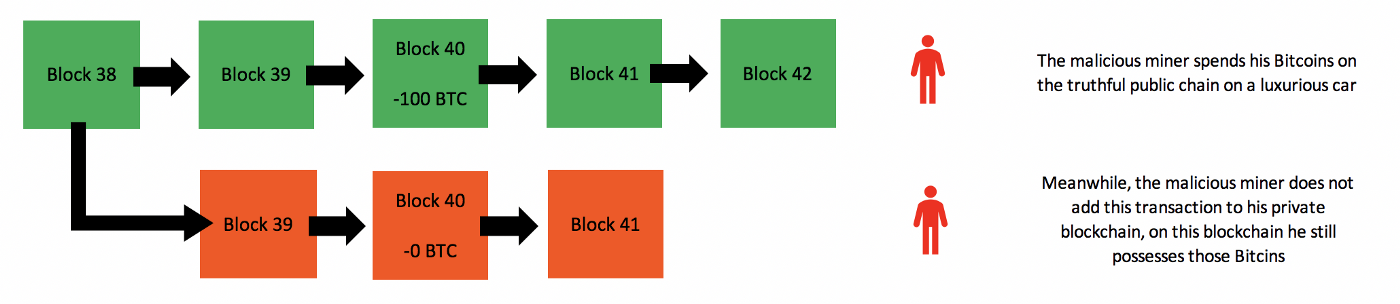
\includegraphics[width=1\linewidth]{../img/attack_1.png}
      \end{figure}
      \begin{figure}
          \centering
          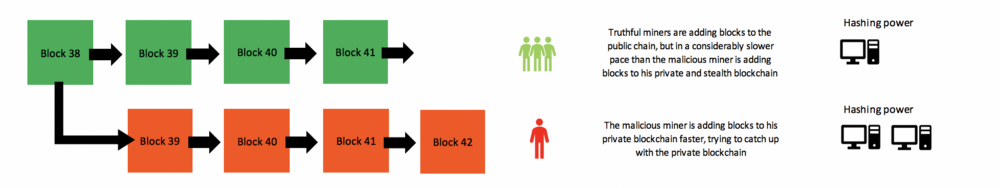
\includegraphics[width=1\linewidth]{../img/attack_2.png}
      \end{figure}
  \end{frame}
  
  
  
  \section{Anonimità in Bitcoin}
  \subsection{Problemi di anonimità}
  \begin{frame}{Problemi di anonimità}
      \begin{itemize}
          \item Le transazioni avvengono tra indirizzi (``pseudonimi'')
          \item Gli indirizzi non sono abbastanza per assicurare la privacy degli utenti
          \begin{itemize}
              \item[-] le transazioni sono pubbliche 
              \item[-] transazioni = ``catene'' di firme digitali
              \item[-] le transazioni possono essere collegate tra loro (e.g. tramite analisi behaviour-based): singola transazione collegata all'identità dell'utente \MVRightarrow\, tutte le sue transazioni sono esposte
          \end{itemize}
          \item Soluzione (parziale): ricevere pagamenti usando solo indirizzi nuovi (evitare address reuse) 
          \begin{itemize}
              \item[-] non sufficiente per garantire la privacy  
          \end{itemize}
          %\item Analogia con le banche: estratto conto bancario pubblico ma con i nomi oscurati
      \end{itemize}
  \end{frame}
  
  
  
  \begin{frame}{Problemi di anonimità}
  \framesubtitle{Esempi di compromissione della privacy}
      \begin{enumerate}
          \item \textbf{Sfruttare le transazioni multi-input}
          \begin{itemize}
              \item transazione multi-input = transazione che accetta in input più UTXOs 
              \item gli UTXOs in input appartengono a indirizzi diversi \MVRightarrow\, quegli indirizzi appartengono allo stesso utente
          \end{itemize}
          \pause
          \item \textbf{Sfruttare gli indirizzi shadow}
          \begin{itemize}
              \item indirizzo shadow = indirizzo automaticamente creato per raccogliere il resto di una transazione
              \item una transazione ha $n$ indirizzi in output, di cui solo uno è un indirizzo nuovo \MVRightarrow il nuovo indirizzo è un indirizzo shadow dell'utente che ha generato la transazione
              \item Soluzione: evitare address reuse 
          \end{itemize}
          \pause
          \item \textbf{Analisi behaviour-based}
          \begin{itemize}
              \item algoritmi di clustering (KMC, HAC) sono stati testati in un ambiente Bitcoin simulato \cite{androulaki2013evaluating}
              \item sono stati in grado di catturare il 43\% dei profili utente con un'accuratezza dell'80\% 
          \end{itemize}
      \end{enumerate}
  \end{frame}
  
  
  
  \begin{frame}{Problemi di anonimità}
      \begin{block}{Tainted bitcoins}
        \begin{itemize}
            \item la storia di ciascun bitcoin può essere tracciata
            \item conseguenza della mancanza di anonimità
            \item alcuni bitcoin possono essere marcati come \textbf{tainted}
            \begin{itemize}
                \item gli utenti sono meno propensi ad accettarli \MVRightarrow\, deflazione del loro valore
            \end{itemize}
        \end{itemize}
      \end{block}
  \end{frame}
  
  
  
  
  \begin{frame}{Aumentare l'anonimità di Bitcoin}
      Come amentare l'anonimità in Bitcoin? Due principali approcci:
      \begin{enumerate}
          \item Mixing services
          \begin{itemize}
              \item[\MVRightarrow] efficienti
              \item[\MVRightarrow] richiedono fiducia assoluta in una terza parte
          \end{itemize}
          \item Estensioni crittografiche di Bitcoin
          \begin{itemize}
              \item[\MVRightarrow] non richiedono fiducia in parti terze
              \item[\MVRightarrow] performance inferiori
              \item[\MVRightarrow] nuove crittovalute \footnote{e.g. ZeroCoin \cite{miers2013zerocoin} e ZeroCash \cite{sasson2014zerocash}} o estensioni Bitcoin-compatible (soft-fork)
          \end{itemize}
      \end{enumerate}
  \end{frame}
  
  
  \subsection{Mixing Services}
  \begin{frame}{Mixing Services}
      \begin{figure}
          \centering
          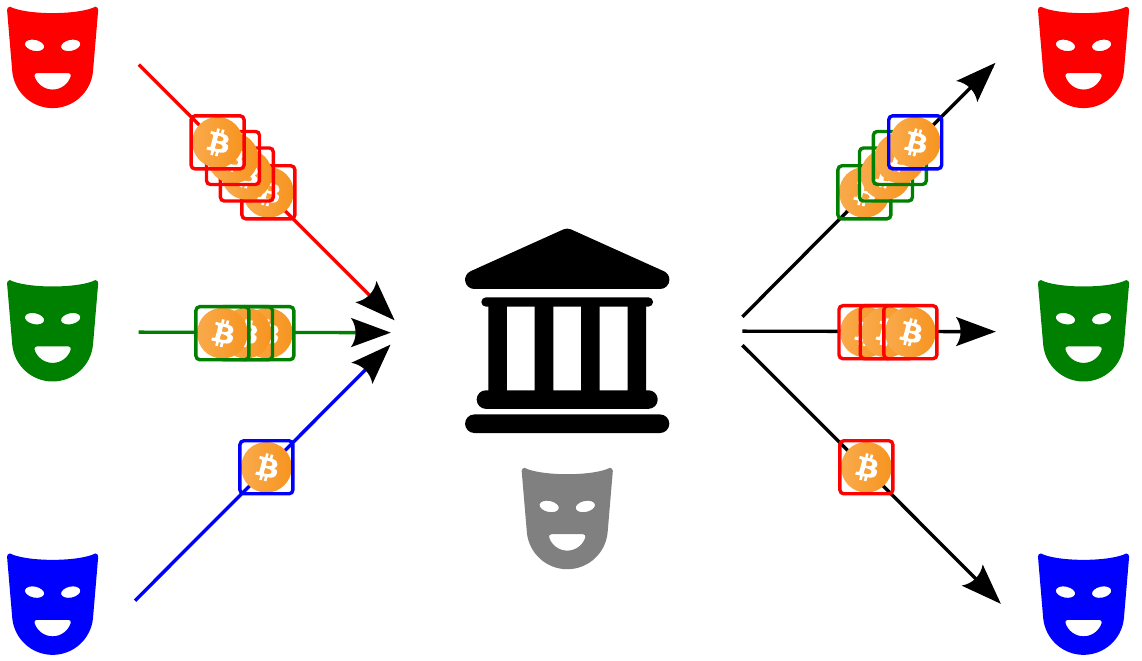
\includegraphics[width=0.6\linewidth]{../img/mixing-service-scheme.png}
      \end{figure}
      \begin{itemize}
          \item Mediatori che trasferiscono pagamenti da un insieme di indirizzi in input a un insieme di indirizzi in output
          \item Il trasferimento viene fatto tale che sia difficile risalire a ``chi ha pagato chi''
      \end{itemize}
  \end{frame}
  
  
  
  \begin{frame}{Mixing Services}
      Esempi Mixing Services: 
      \begin{itemize}
          \item Mixcoin
          \begin{itemize}
              \item[-] si appoggia a una singola parte terza \MVRightarrow non così sicuro (e.g. la parte terza può potenzialmente rubare i bitcoins) 
          \end{itemize}
          \item CoinParty
          \begin{itemize}
              \item[-] si appoggia su più parti terze
              \item[-] considerato sicuro solo se $2/3$ delle parti sono oneste
          \end{itemize}
      \end{itemize}
  \end{frame}
  
  
  \subsection{Schemi di anonimità Bitcoin-compatible}
  \begin{frame}{Scenario di riferimento}
      \begin{itemize}
          \item $A$ vuole mandare 1 bitcoin a $B$ in modo anonimo          \item se $A$ invia 1 BTC da $address_A$ (posseduto da $A$) a $address_B$ (posseduto da $B$) allora nella Blockchain viene generato un record che collega i due indirizzi tra loro
          \begin{itemize}
              \item[-] i collegamenti tra indirizzi possono essere usati per de-anonimizzare gli utenti
              \item[-] usare nuovi indirizzi per ciascun pagamento ricevuto non è sufficiente
          \end{itemize} \pause 
          \item Soluzione:
          \begin{minipage}{\linewidth}
            \includegraphics[width=0.4\linewidth]{../img/scenario.png}
          \end{minipage}
          \item $I$ rompe il collegamento tra gli indirizzi usati da $A$ e $B$
          \begin{itemize}
              \item agisce di fatto come un mixing service, ma non è richiesta fiducia
          \end{itemize}
      \end{itemize}
  \end{frame}
  
  
  
  \begin{frame}{Blind Signatures}
      \begin{itemize}
          \item Introdotte da David Chaum nel 1982 \cite{chaum1982blind}
          \item Primitiva crittografica che permette a un'entità di firmare un messaggio senza essere in grado di leggerlo
          \item Analogia: busta con carta carbone al suo interno 
      \end{itemize}
      
      \pause
      \begin{block}{RSA Blind Signature scheme}
        \begin{itemize}
            \item Blinding factor $b=r^{e}\bmod n$, con $r$ numero casuale
            \item Il messaggio $m$ è oscurato con $b$: $m_{*}=b\cdot m\bmod n$
            \item $m_*$ viene mandato al firmatario. Il firmatario lo firma calcolando $s_*$: \[ s_*=m_*^d\bmod n = b^d\cdot m^d\bmod n = r^{e\cdot d}\cdot m^d \bmod n = r\cdot m^d \bmod n \]
            \item L'utente può dividere $s_*$ per $r$ al fine di ottenere $s=m^d\bmod n$, ossia la firma RSA sul messaggio $m$
        \end{itemize}
      \end{block}
  \end{frame}
  
  
  
  \begin{frame}{Primo schema: schema di eCash}
      \begin{figure}
          \centering
          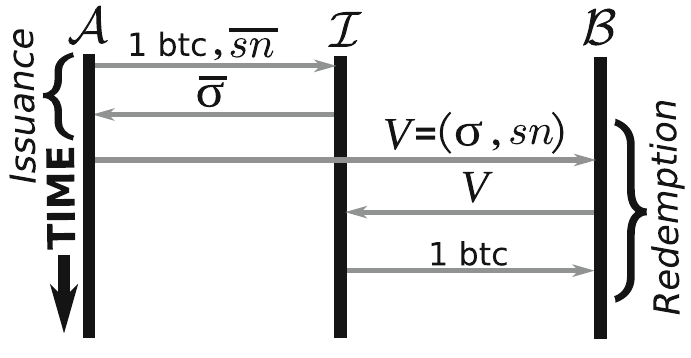
\includegraphics[width=0.6\linewidth]{../img/eCash-scheme.png}
      \end{figure}
      \begin{itemize}
          \item Concepito da David Chaum per eCash (una crittovaluta anonima) nel 1982 \cite{chaum1982blind}
          \item $I$ non conosce chi $A$ vole pagare \pause
          \item \red{Problema principale}: $I$ deve esseere onesto
          \begin{itemize}
              \item[-] un $I$ maligno potrebbe rifiutarsi di emettere il voucher ad $A$
          \end{itemize}
          \pause
          \item \textcolor{green}{Soluzione}: schema di Heilman \cite{heilman-blindly-signed-contracts}
      \end{itemize}
  \end{frame}
  
  
  
  
  \begin{frame}{Secondo schema: schema di Heilman}
      \begin{figure}
          \centering
          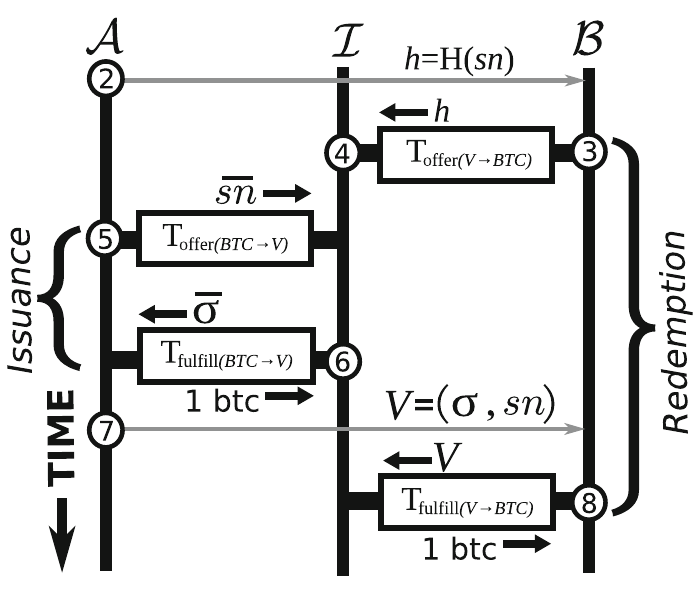
\includegraphics[width=0.4\linewidth]{../img/heilman-scheme.png}
      \end{figure}
      \begin{itemize}
          \item Utilizza \emph{transaction contracts} per implementare due \emph{fair exchange}
        %  \begin{itemize}
         %     \item[\MVRightarrow] \textbf{idea base}: $A$ trasferisce un bitcoin ad $I$ se e solo se riceve in cambio un voucher $V$ valido
         % \end{itemize}
          \item Composto da 4 transazioni (confermate in 3 blocchi della Blockchain) che implementano 2 fair exchange
      \end{itemize}
  \end{frame}
  
  
  
  
  \begin{frame}{Secondo schema: schema di Heilman (Cont. 1)}
      \begin{figure}
          \centering
          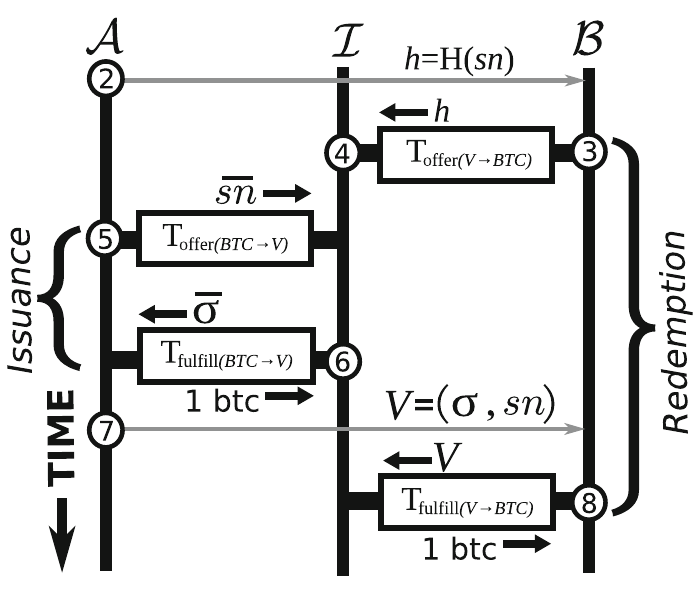
\includegraphics[width=0.4\linewidth]{../img/heilman-scheme.png}
      \end{figure}
      \begin{block}{1) Fair-exchange $V\rightarrow BTC$}
        \begin{itemize}
            \item Interazione tra $B$ ed $I$
            \item Composto dalle transazioni $T_{offer(V\rightarrow BTC)}$ e $T_{fullfill(V\rightarrow BTC)}$
            \item Garantisce che un $I$ maligno non possa ricevere il voucher di $B$ senza in cambio fornirgli un bitcoin
        \end{itemize}
      \end{block}
  \end{frame}
  
  
  
  
  \begin{frame}{Secondo schema: schema di Heilman (Cont. 2)}
      \begin{figure}
          \centering
          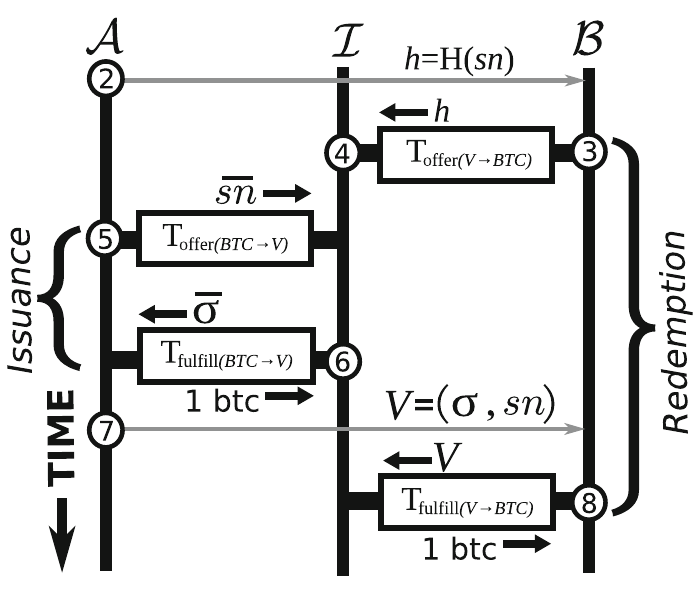
\includegraphics[width=0.4\linewidth]{../img/heilman-scheme.png}
      \end{figure}
      \begin{block}{2) Fair-exchange $BTC\rightarrow V$}
        \begin{itemize}
            \item Interazione tra $A$ ed $I$
            \item Composto dalle transazioni $T_{offer(BTC\rightarrow V)}$ e $T_{fullfill(BTC\rightarrow V)}$
            \item Garantisce che un $I$ maligno non possa ricevere il bitcoin da $A$ senza fornirgli in cambio il voucher $V$
        \end{itemize}
      \end{block}
  \end{frame}
  
  
  
  \begin{frame}{Secondo schema: schema di Heilman (Cont. 3)}
      \begin{block}{Implementazione del fair-exchange $BTC\rightarrow V$}
        \begin{itemize}
            \item Implementato tramite \emph{transaction contract} (Script)
            \begin{itemize}
                \item[\MVRightarrow] ciascuna transazione è associata ad un insieme di regole richieste per spendere l'output della transazione
            \end{itemize}
            \item CHECK\_LOCK\_TIME\_VERIFY usato per bloccare temporalmente la transazione
            \item $A$ genera $T_{offer(BTC\rightarrow V)}$. L'output potrà essere speso in una futura transazione $T_f$ solo se:
            \begin{enumerate}
                \item $T_f$ è firmata da $I$ e contiene una valida blind signature $\overline\sigma$ su $\overline{sn}$
                \item[] OPPURE 
                \item $T_f$ è firmata da $A$ e la time window $Tw$ è scaduta
            \end{enumerate}
        \end{itemize}
      \end{block}
      \pause
      
      L'implementazione del fair-exchange $BTC\rightarrow V$ è analoga
  \end{frame}
  
  
  
  
  \begin{frame}{Secondo schema: schema di Heilman (Cont. 4)}
      \begin{figure}
          \centering
          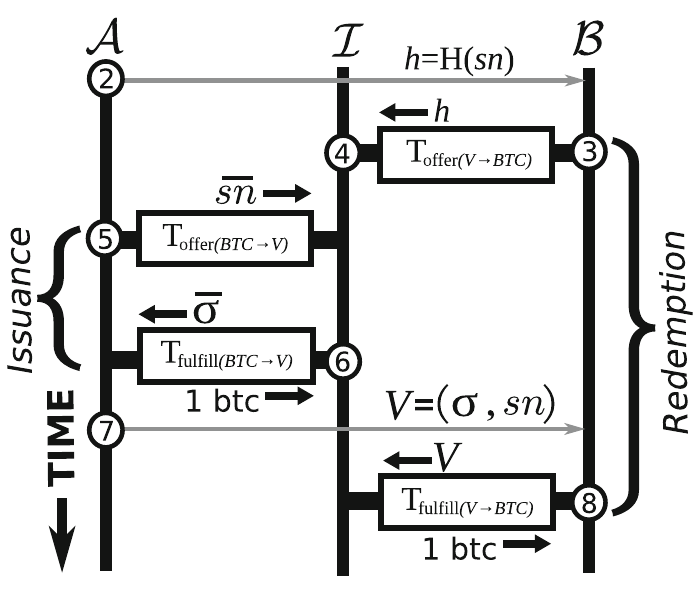
\includegraphics[width=0.4\linewidth]{../img/heilman-scheme.png}
      \end{figure}
      
      \begin{enumerate}
          \item $B$ crea un nuovo indirizzo effimero per ricevere il pagamento \pause
          \item $A$ scegli un $sn$ casuale, calcola $h=H(sn)$ ed invia $h$ a $B$ \pause
          \item $B$ invia $h$ ad $I$ e gli chiede di creare il contratto $T_{offer(V\rightarrow BTC)}$
          \begin{itemize}
              \item[\MVRightarrow] $I$ offre ad $B$ 1 BTC sotto la condizione che $B$ fornisca un voucher $V$ valido con numero seriale $sn$ t.c. $h=H(sn)$ entro il tempo $tw2$
          \end{itemize}
      \end{enumerate}
  \end{frame}
  
  
  
  
   \begin{frame}{Secondo schema: schema di Heilman (Cont. 5)}
      \begin{figure}
          \centering
          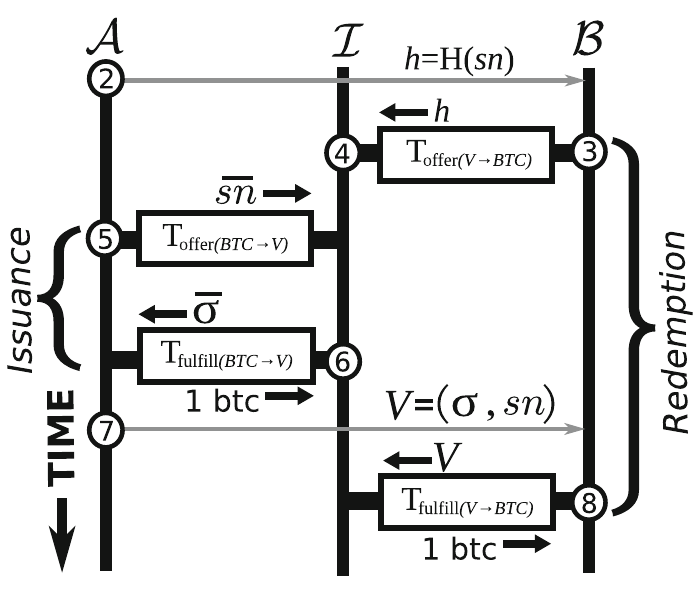
\includegraphics[width=0.4\linewidth]{../img/heilman-scheme.png}
      \end{figure}
      
      \begin{enumerate}
      \setcounter{enumi}{3}
          \item Se $h$ non è già stato usato, allora $I$ crea il contratto richiesto da $B$ e lo pubblica nella Blockchain \pause
          \item $A$ oscura $sn$ e ottiene $\overline{sn}$, poi attende che $T_{offer(V\rightarrow BTC)}$ venga confermata. Quando questo avviene, $A$ crea il contratto $T_{offer(BTC\rightarrow V)}$
          \begin{itemize}
              \item[-] offre $1+w$ bitcoin, con $w$=ricompensa per $I$
          \end{itemize}
      \end{enumerate}
  \end{frame}
  
  
  
  
  \begin{frame}{Secondo schema: schema di Heilman (Cont. 6)}
      \begin{figure}
          \centering
          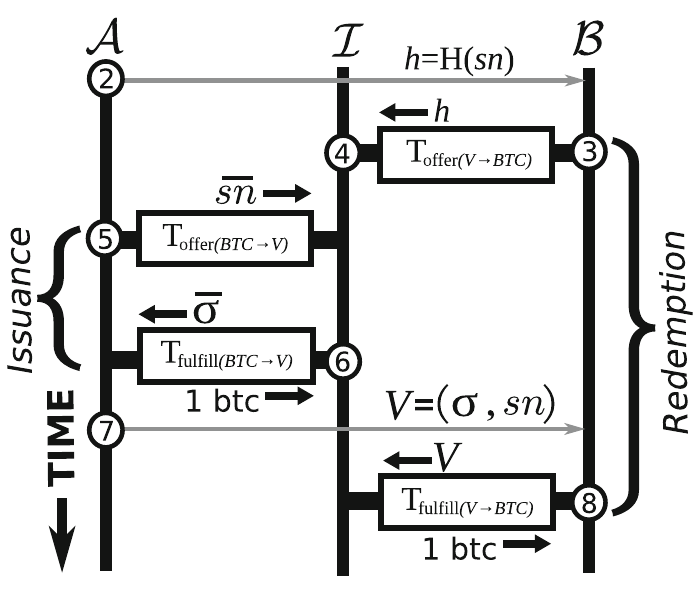
\includegraphics[width=0.4\linewidth]{../img/heilman-scheme.png}
      \end{figure}
      
      \begin{enumerate}
      \setcounter{enumi}{5}
          \item $I$ aspetta che $T_{offer(BTC\rightarrow V)}$ venga confermata. Quando questo avviene, $I$ completa il fair exchange creando $T_{fullfill(BTC\rightarrow V)}$
          \item $A$ legge $\overline{\sigma}$ dalla transazione e invia $V=(\sigma,sn)$ a $B$
      \end{enumerate}
  \end{frame}
  
  
  
  
  \begin{frame}{Secondo schema: schema di Heilman (Cont. 7)}
      \begin{figure}
          \centering
          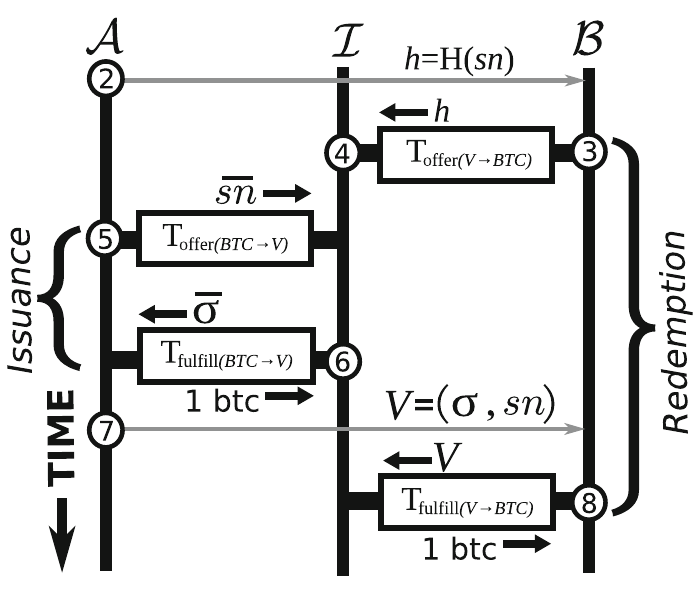
\includegraphics[width=0.4\linewidth]{../img/heilman-scheme.png}
      \end{figure}
      
      \begin{enumerate}
      \setcounter{enumi}{7}
          \item $B$ completa il fair exchange creando $T_{fullfill(V\rightarrow BTC)}$, la quale contiene $V$
      \end{enumerate}
  \end{frame}
  
  
  
  \begin{frame}{Considerazioni sull'anonimità dello schema}
      \begin{figure}
          \centering
          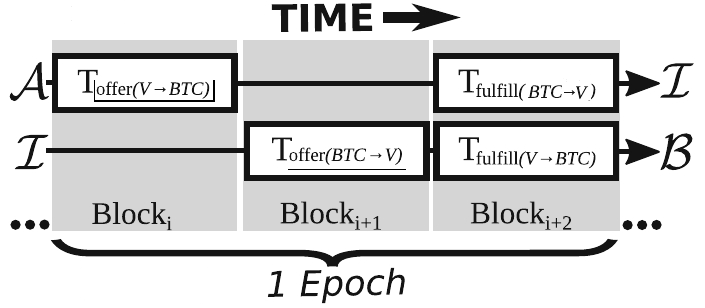
\includegraphics[width=0.4\linewidth]{../img/epochs.png}
      \end{figure}
      \begin{itemize}
          \item Le 4 transazioni sono confermate e memorizzate in un'epoca
          \item L'anonimità dipende dal numero di pagamenti effettuati attraverso $I$ in una determinata epoca
      \end{itemize}
  \end{frame}
  
  
  
  
  \begin{frame}{Considerazioni sull'anonimità dello schema (Cont. 1)}
      Valgono le seguenti assunzioni: 
      \begin{enumerate}
          \item gli utenti si coordinano al fine di rispettare la disposizione in epoche delle transazioni (e.g. scelta del blocco iniziale come blocco con altezza multiplo di 3) 
          \item $A$ e $B$ si fidano tra loro 
          \begin{itemize}
              \item[-] se $A$ o $B$ fossero maligni allora uno di loro potrebbe cospirare con $I$
          \end{itemize}
          \item $B$ riceve i pagamenti usando sempre indirizzi nuovi
          \item i pagatori effettuano un solo pagamento per epoca; i beneficiari accettano un solo pagamento per epoca
      \end{enumerate}
      \pause
      \begin{block}{}
      Assunzioni 2 + 3 \MVRightarrow\, in ciascuna epoca vi sono $n$ indirizzi che effettuano pagamenti ed $n$ indirizzi che ricevono pagamenti
      \begin{itemize}
          \item[\MVRightarrow] $1/n$ di probabilità di collegare un pagatore $A$ ad un beneficiario $B$
      \end{itemize}
      \end{block}
  \end{frame}
  
  
  \begin{frame}{Considerazioni sull'anonimità dello schema (Cont. 2)}
      \begin{block}{Perchè $B$ deve usare indirizzi nuovi?}
          \begin{itemize}
              \item Impedisce ad $I$ di deanonimizzare $A$ e $B$ annullando lo scambio
              \item Esempio:
                \begin{itemize}
                    \item[-] $I$ rifiuta di rilasciare il Voucher $V$ ad $A$ (non effettua $T_{fullfill(BTC\rightarrow V)}$)
                    \item[-] $A$ non ottiene il voucher \MVRightarrow\, non può inviare $V$ a $B$ 
                    \item[-] $B$ non è in grado di effettuare $T_{fullfill(V\rightarrow BTC)}$
                    \item[\MVRightarrow] $I$ può fare il match tra gli scambi con $A$ annullati e gli scambi non completati con $B$ 
                \end{itemize}
                \pause
               \item Esempio 2:
               \begin{itemize}
                   \item[-] $I$ si rifiuta di rilasciare il Voucher $V$ a tutti tranne $A$
                   \item[-] $I$ può identificare $B$ come l'unico che soddisfa il contratto 
               \end{itemize}
               \pause
               \item \textcolor{green}{Soluzione}:
               \begin{itemize}
                   \item[-] $B$ può accorgersi di questi attacchi 
                   \item[-] quando si accorge scarta l'indirizzo (effimero) compromesso 
               \end{itemize}
          \end{itemize}
      \end{block}
  \end{frame}
  
  
  
  \begin{frame}{Considerazioni sull'anonimità dello schema (Cont. 3)}
      \begin{itemize}
          \item Gli utenti conoscono la dimensione del loro set di anonimità ($n$) osservando la Blockchain dopo che le transazioni sono state completate
          \item Cosa fare se $B$ ritiene che il suo $n$ sia troppo piccolo? \pause
          \begin{itemize}
              \item[-] si assume che $B$ sia stato pagato all'indirizzo $address_B$
              \item[-] $B$ crea un nuovo indirizzo effimero $address_B'$
              \item[-] $B$ paga $address_B$ a $address_B'$ in un'altra epoca
          \end{itemize}
      \end{itemize}
  \end{frame}
  
  
  
  
  
  \section{Scalabilità di Bitcoin}
  \subsection{Overview}
  \begin{frame}{Panoramica della scalabilità di Bitcoin}
      \begin{itemize}
          \item Bitcoin viene usato sempre di più \MVRightarrow\, la sua abilità di scalare ha ultimamente ricevuto parecchie attenzioni
          \item Principali preoccupazioni:
          \begin{enumerate}
              \item possono le crittovalute basate su Blockchain scalare e raggiungere le performance dei tradizionali processori di pagamenti? (e.g. Visa)
              \item come fare per raggiungere tali performance? 
          \end{enumerate}
          \pause
          \item Performance attuali di Bitcoin: 
          \begin{itemize}
              \item circa 10 min per confermare una transazione 
              \item dimensione massima del blocco = 1 MB (dimensione media = 800 KB) \cite{current-block-size}
              \item throughput massimo = 7 transazioni/sec \cite{wikipedia_scalability_2018}
              \item throughput limitato dalla dimensione massima del blocco e dal tempo con cui i blocchi vengono prodotti (block interval)
          \end{itemize} \pause
          \item Confronto con Visa:  \cite{wikipedia_scalability_2018}
          \begin{itemize}
              \item 2000 transazioni/sec in media 
              \item picchi di 56 000 transazioni/sec
          \end{itemize}
      \end{itemize}
  \end{frame}
  
  
  
  
  
  \begin{frame}{Panoramica della scalabilità di Bitcoin (Cont. 1)}
      \begin{itemize}
          \item Idea per aumentare il throughput: \textbf{riparametrizzazione}
          \begin{itemize}
              \item[-] diminuire il block interval
              \item[-] aumentare la dimensione massima dei blocchi (attualmente 1 MB)
          \end{itemize}
          \item Grande dibattito 
          \begin{itemize}
              \item[\MVRightarrow] \textcolor{red}{Principale svantaggio}: minore decentralizzazione
              \item[\MVRightarrow] meglio ottimizzare l'uso dello spazio disponibile attuale
          \end{itemize}
          \item In \cite{croman-scaling-blockchain}, l'autore dimostra che: 
          \begin{itemize}
              \item[-] la riparametrizzazione da sola non basta per scalare Bitcoin
              \begin{itemize}
                  \item[\MVRightarrow] limitazioni sui parametri
                  \item[\MVRightarrow] presenza di bottleneck all'interno del sistema Bitcoin
              \end{itemize}
          \end{itemize}
      \end{itemize}
  \end{frame}
  
 
  
  
  
  \subsection{Limitazioni della riparametrizzazione}
  \begin{frame}{Definizione di alcune metriche}
      \begin{enumerate}
          \item ``X\% block propagation delay'' = tempo richiesto affinchè il X\% dei nodi riceva completamente un blocco
          \begin{itemize}
              \item[\MVRightarrow] calcolato empiricamente
          \end{itemize}
          \item $\text{``X\% effective throughput''} = \frac{\text{block size}}{\text{X\% block propagation delay}}$
      \end{enumerate}
      \begin{itemize}
          \item transaction rate $>$ X\% effective throughput $\rightarrow$ (100 -X)\% dei nodi saranno di fatto inattivi
      \end{itemize}
  \end{frame} 
  
  
  \begin{frame}{Limiti}
    Premesse:
    \begin{itemize}
        \item si vuole mantenere il livello corrente di decentralizzazione 
        \begin{itemize}
            \item[\MVRightarrow] almeno 90\% dei nodi devono funzionare correttamente
        \end{itemize}
        \item viene utilizzata la rete peer-to-peer attuale di Bitcoin, senza alcuna modifica
        \begin{itemize}
            \item[\MVRightarrow] una qualunque modifica cambierebbe il valore di X\% effective throughput
        \end{itemize}
    \end{itemize}
    
    \begin{block}{Limite sulla dimensione massima del blocco}
        \[ \text{90\% block propagation delay} < \text{block interval} \]
        ossia 
        \[ \frac{\text{block size}}{\text{90\% effective throughput}} < \text{block interval} \]
        \begin{itemize}
            \item[\MVRightarrow] \footnote{assumendo block interval = 10 min} dimensione massima non superiore a 4 MB
        \end{itemize}
    \end{block}
  \end{frame}
  
  
  
  
  \begin{frame}{Limiti (Cont. 1)}
      \begin{block}{Limiti sul block interval}
        \begin{itemize}
            \item ridurre block interval = ridurre latenza 
            \item ridurre block interval \MVRightarrow\, anche la dimensione del blocco deve essere ridotta (si veda equazione limite throughput)
            \item Dimensione del blocco troppo piccola \MVRightarrow\, la banda della rete non viene usata a pieno
            \item Risultati ottenuti da \cite{croman-scaling-blockchain} effettuando esperimenti/misurazioni: il block interval non deve essere inferiore a 12 secondi al fine di:
            \begin{itemize}
                \item[-] avere almeno il 90\% di effective throughput
                \item[-] utilizzare a pieno la banda disponibile
            \end{itemize}
        \end{itemize}
      \end{block}
  \end{frame}
 
 
 
 
 
  \subsection{Analisi dei bottleneck}
  \begin{frame}{Network Plane}
      \begin{itemize}
          \item Funzione: propagare le transazioni valide
          \item Bitcoin non utilizza a pieno la banda disponibile
          \item Due principali inefficienze: 
          \begin{enumerate}
              \item prima di propagare una transazione, i nodi devono riceverla completamente e validarla (prevenzione DoS)
              \begin{itemize}
                  \item[\MVRightarrow] \textcolor{green}{soluzione possibile}:
                  protocolli di broadcas a bassa latenza + permettere ai nodi di limitare le trasmissioni dai loro peer
              \end{itemize}
              \pause
              \item le transazioni vengono propagate (creazione dei pool), poi anche i blocchi vengono propagati: alcune transazioni vengono trasmesse 2 volte
              \begin{itemize}
                  \item[\MVRightarrow] \textcolor{green}{soluzione possibile}: set reconciliation protocol (i pool di transazioni dei singoli nodi sono simili) 
              \end{itemize}
          \end{enumerate}
      \end{itemize}
  \end{frame}
  
  
  
  \begin{frame}{Consensus Plane}
      \begin{itemize}
          \item Funzione: mining e raggiungimento del consenso
          \item Limitazione: Proof of Work 
          \begin{itemize}
              \item[-] compromesso tra velocità di consenso e sicurezza
          \end{itemize}
          \item \textcolor{green}{Possibile soluzione}: utilizzare meccanismi di consenso alternativi (e.g. Proof of Stake) 
      \end{itemize}
  \end{frame}
  
  
  
  
  \begin{frame}{Storage Plane}
      \begin{itemize}
          \item Funzione: memorizzare il libro mastro di Bicoin e permettere le operazioni \texttt{read} and \texttt{write} su di esso
          \item Principale problema: ciascun nodo memorizza una copia dell'intera Blockchain
          \begin{itemize}
              \item[-] in Giugno 2018 la dimensione era di 178 GB \cite{statista}
              \item[-] la dimensione cresce esponenzialmente
          \end{itemize}
      \end{itemize}
  \end{frame}
  
  
  
  
  \begin{frame}{View Plane}
      \begin{itemize}
          \item Funzione: permettere ai miner di minare senza dover memorizzare una copia dell'intera Blockchain
          \begin{itemize}
              \item[-] operano su una \emph{view} del libro mastro: UTXO set
              \item[-] l'UTXO set specifica il saldo corrente di tutte le entità
              \item[-] UTXO deve essere calcolato
          \end{itemize}
          \item Problema principale: calcolare la view richiede molto tempo
          \item \textcolor{green}{Soluzione possibile}: memorizzare la view nello Storage Plane
      \end{itemize}
  \end{frame}
  
  
  
  
  \section{Conclusioni}
  \begin{frame}{Contents}
      \frametitle{\contentsname}
    \begin{multicols}{2}
        \tableofcontents[currentsection,currentsubsection]
    \end{multicols}
  \end{frame}
  
  
  
  \begin{frame}{Conclusioni}
      \begin{itemize}
          \item Blockchain: tecnologia sempre più popolare 
          \item Soluzione di ogni problema?  
          \begin{itemize}
              \item[-] bisogno di un database condiviso? 
              \item[-] i dati del DB cambiano frequentemente ed è necessario poter verificare la storia di ciascun dato? 
              \item[-] i dati trattati sono riservati? 
              \item[-] più entità che leggono/scrivono nel DB? 
              \item[-] le parti coinvolte non sono fidate? 
              \item[-] possono i dati essere controllati da un'unica entità centrale fidata? 
              \item[-] quanto sono importanti le performance? 
              \item[-] ...
              \item[\MVRightarrow] \textcolor{orange}{dipende dall'applicazione e dal contesto} 
          \end{itemize}
          \pause
          \item Ideale per crittovalute
      \end{itemize}
  \end{frame}
  
  
  
  
  \begin{frame}{Conclusioni}
      \begin{itemize}
          \item Bitcoin: prima reale applicazione di Blockchain
          \item Diversi vantaggi rispetto alle valute tradizionali 
          \begin{itemize}
              \item[-] no autorità centrali 
              \item[-] trasparenza
              \item[-] sicurezza
              \item[-] maggiore anonimità
          \end{itemize}
      \end{itemize}
  \end{frame}
  
  
  \begin{frame}{Conclusioni}
     \begin{itemize}
          \item Problema scalabilità
          \item Problema anonimità 
          \begin{itemize}
              \item[-] risolvibile (mixing services, schemi, estensioni, etc.) 
              \item[-] esistono altre crittovalute appositamente progettate per garantire privacy (Monero \cite{getmonero}, ZCash \cite{zcash}, ...)  
          \end{itemize}
          \item Altri problemi vari
          \begin{itemize}
              \item[-] scalabilità \& performance
              \item[-] anonimità 
              \item[-] Proof-of-Work
              \item[-] supporto limitato a smart contract 
          \end{itemize}
          \pause
          \item Numerose crittovalute alternative. Più diffusa: Ethereum
          \begin{itemize}
              \item[-] supporta smart contracts (linguaggio di programmazione Turing completo)
              \item[-] permette di realizzare applicazioni distribuite 
          \end{itemize}
      \end{itemize}
  \end{frame}
  
  \begin{frame}{Conclusioni}
      \centering \Huge
      \emph{Grazie per l'attenzione}
  \end{frame}
  


  \begin{frame}[allowframebreaks]{References}
    \printbibliography
  \end{frame}

\end{document}
